The first step of encryption begins at the sender's iOS device when the device
generates two key pairs\cite{apple}.  The first is a 1280-bit key used for encrypting the
message itself using an RSA encryption algorithm.  The second key is a 256-bit
ECDSA key used for signing the message so the receiver can verify the message
was sent from the correct device.  Both RSA and ECDSA 
belong to a class of encryption algorithms known as public-key encryption or
also known as asymmetric cryptography\cite{trappe}. In a public-key cryptosystem, two pairs
of keys are generated.  One of the keys is known as the public key.  This key
is used for encrypting the plaintext, or the actual message itself, but it does
so in such a way that it is effectively impossible to use the public key to
decrypt the message.  This property of the public key means it poses no
security risk for others to know of the key, hence the name \textit{public}.  In
contrast, the private key can only be used to decrypt ciphertext that has been
encrypted with the corresponding public key.  Thus, the private key must be
only known to the intended receiver of the message in order to guarantee
security of the message.  Returning to iOS, when the two key pairs are
generated, the device stores the private keys locally, in a secure area of the
device.  It then sends the two public keys to the Apple Push Notification
Service Service (APNS) where they are associated with the device's phone number.
The public keys of any receiver can then be pushed down to any device
requesting to send an iMessage to another iOS device\cite{apple}.

The second step is actually sending the iMessage which begins by adding
recipients of the iMessage.  The sender's iOS device finds the phone numbers of
the recipients in its local Contact list and performs a request against the
APNS server, asking for the public keys associated with the phone numbers of
the recipients\cite{apple}.  This contact with the server is the first opportunity for
attack that we see so far.  Both the server and the sender's device need to
know that their communication is uninterrupted.  It is possible for the
sender's device to send a message to a third-party, a malicious receiver who,
upon reading the message, then forwards the information along to the APNS
server so it looks like there was no interruption of communication.  Such an
attack is known as a Man-in-the-middle attack due to the malicious third party
in the middle of the communication.  To ensure a secure communication between
the device and APNs, communication is encrypted using the TLS algorithm
discussed earlier.  Once the connection has been established, APNS pushes all
the public keys of the recipient devices down to the sender device.  Now the
sender device has all the information it needs to start encrypting the message.

The message itself is encrypted using the Advanced Encryption Standard
algorithm, or AES, in Counter (CTR) mode.  AES was standardized in 2001 for the
specific purpose of encrypting electronic data and, in contrast to RSA and
ECDSA, is part of the category of symmetric key cryptography.  This means that
the same key can be used to both encrypt and decrypt the message.  One caveat
of AES is that it is a block cipher and so can only be used to encrypt blocks
of, in this case, 128-bits.  With each character being represented with 8-bits
this means AES can be used to encrypt only 16 characters at a time!  A mode of
operation is used to securely encrypt many blocks of data using a single block
encryption algorithm.  Apple uses AES in CTR mode which means that each block
is fed a number, or initialization vector, at encryption time.  The next block
to be encrypted is fed the initialization vector plus one.  This continues with
every block being fed the incremented counter used in the previous block.  The
following graphic demonstrates the CTR mode encryption.

\begin{center}
    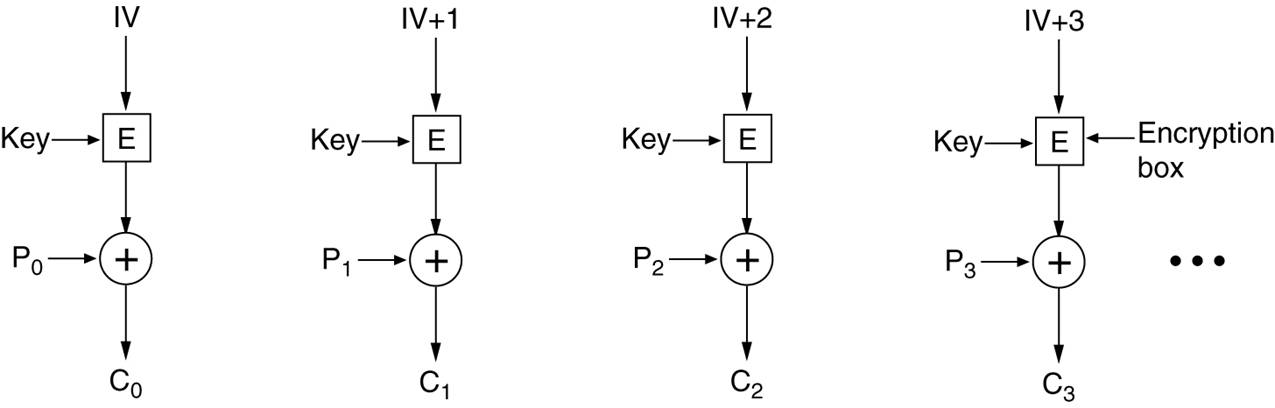
\includegraphics[width=0.75\textwidth]{ctr.jpg}
\end{center}

Interestingly, the data that is encrypted is not actually the plaintext but it
is the counter and the key.  The output of this encryption is then ``added'' to
the plaintext in an XOR operation to produce a block of ciphertext.  This
process allows the entire message to be securely encrypted but this ends up
being not enough security.

In order for the receiver to interpret the message they must also receive the
key used for AES so both the encrypted message and the key must be sent to the
receiver.  This poses another security risk because any unintended recipient
could simply use the key to decrypt the message (AES is symmetric after all).
The conclusion is that the key must also be protected through encryption.
Apple implements this secondary layer of encryption through RSA.  One of the
two public keys pushed down to the sender's device earlier was the receiver's
public RSA key.  The sender's device now clumps the encrypted message, the AES
key, and any necessary padding into one big block which is then encrypted with
RSA.  This chunk of data is now secure to send\ldots almost.  The receiver has
no way of verifying who actually sent the data it is receiving!  Now Apple uses
ECDSA, also discussed earlier, and the public ECDSA key of the receiver to sign
the RSA encrypted data with the sender's information.  The resultant block, the
RSA encrypted data and the ECDSA signature, are now safe to push to APNs.  The
next time the receiver contacts APNs it will get the encrypted message pushed
down to it and will begin a process much like opening a box to find another box
that must be opened.  The receiver uses its private ECDSA key to decrypt the
signature and verify the sender is, in fact, the correct sender.  Then, it uses
its private RSA key to undo the RSA encryption.  This gives the receiver access
to the AES encrypted message and the AES key.  The receiver uses the AES key to
undo the last level of encryption and, finally, the recipient now knows to pick
up milk from the store!
